% Recurring Pipeline Organ Locator Template for Physical AI Systems
% Arguments:
%   \organActive: Number 1..7 corresponding to the active organ in this chapter
%   1: Sensing & Ingestion (Ch 4)
%   2: Perception & Encoders (Ch 4)
%   3: World Models & State (Ch 5)
%   4: Semantic Deliberation (Ch 6)
%   5: Trajectory Decoders (Ch 7)
%   6: Safety Enforcement (Ch 8)
%   7: Governance & Release (Ch 1, 9, 10, 11, 99)

\documentclass[tikz,border=12pt]{standalone}
\usepackage[T1]{fontenc}
\usepackage{tgheros}
\usepackage{sfmath}
\usepackage{amsmath}
\usepackage{tikz}
\usetikzlibrary{arrows.meta,positioning,shapes.geometric,fit,backgrounds,calc}
\usepackage{xcolor}

% Harvard Crimson & ETH Zurich Color Palette
\definecolor{harvardcrimson}{HTML}{A51C30}
\definecolor{ethdarkblue}{HTML}{1F407A}
\definecolor{ethblue}{HTML}{215CAF}
\definecolor{ethpetrol}{HTML}{007A87}
\definecolor{ethbronze}{HTML}{B87333}
\definecolor{ethpurple}{HTML}{5B4B8A}
\definecolor{ethslate}{HTML}{64748B}
\definecolor{cardbg}{HTML}{F8FAFC}
\definecolor{cardborder}{HTML}{CBD5E1}
\definecolor{activebg}{HTML}{FEF2F2}

\newcommand{\organActive}{1} % Default override

\begin{document}
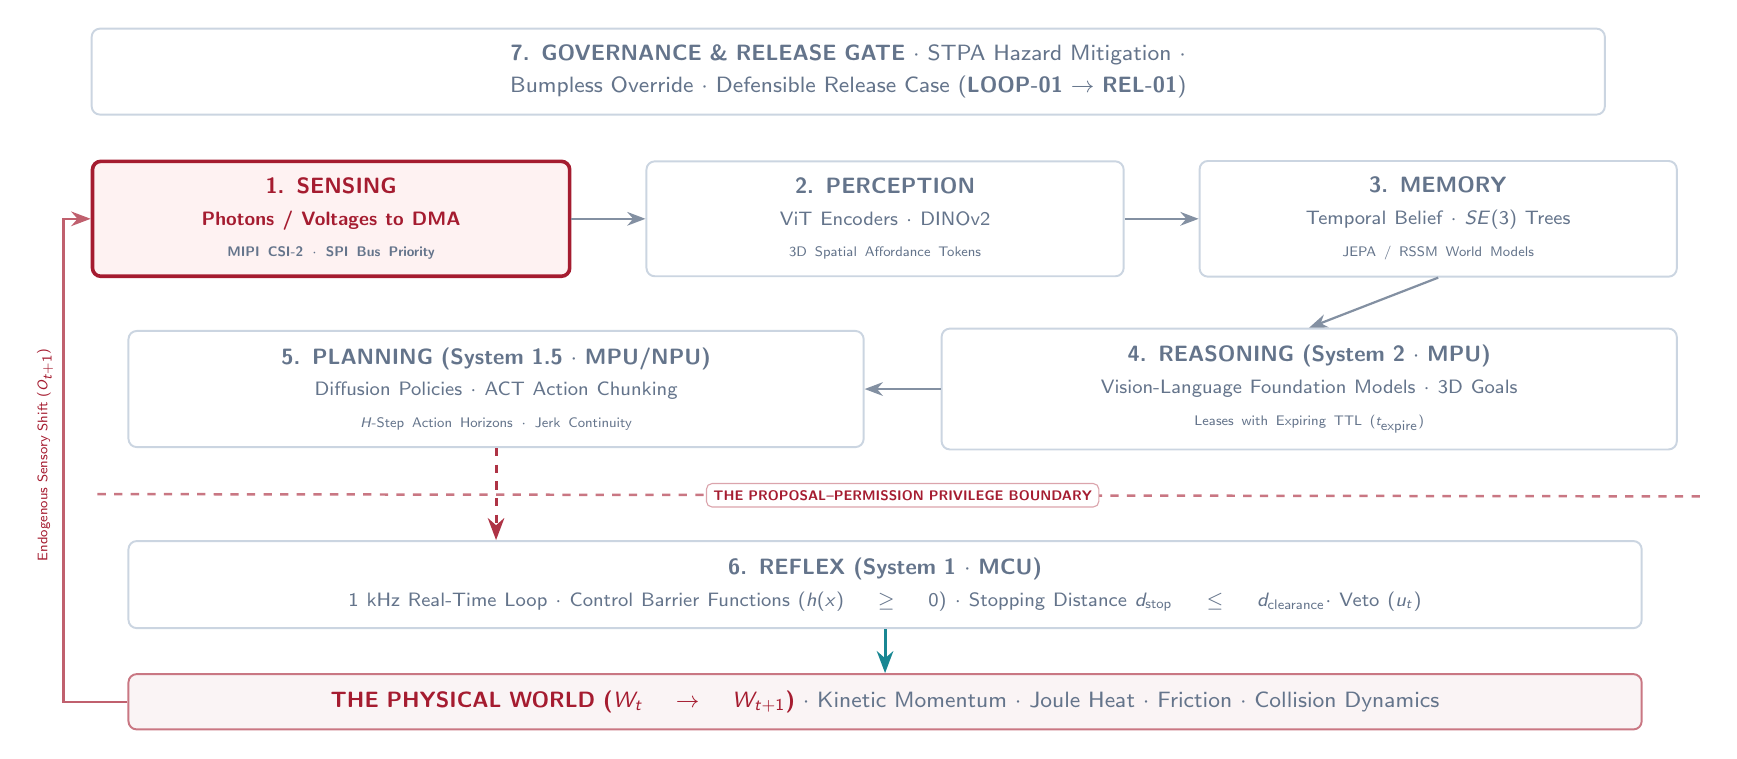
\begin{tikzpicture}[
  font=\sffamily,
  >=Stealth,
  node distance=0.25in,
  baseorgan/.style={
    draw=cardborder,
    fill=white,
    rounded corners=3pt,
    line width=0.7pt,
    inner sep=6pt,
    font=\sffamily\footnotesize,
    align=center,
    text=ethslate
  },
  activeorgan/.style={
    draw=harvardcrimson,
    fill=activebg,
    rounded corners=3pt,
    line width=1.3pt,
    inner sep=6pt,
    font=\sffamily\footnotesize\bfseries,
    align=center,
    text=harvardcrimson
  }
]

  % Top Banner: Stage 7 Governance
  \ifnum\organActive=7
    \node[activeorgan, text width=7.4in] (s7) {
      \textbf{7. GOVERNANCE \& RELEASE GATE} $\cdot$ STPA Hazard Mitigation $\cdot$\\[2pt]
      \mbox{Bumpless Override} $\cdot$ Defensible Release Case (\textbf{LOOP-01} $\to$ \textbf{REL-01})
    };
  \else
    \node[baseorgan, text width=7.4in] (s7) {
      \textbf{7. GOVERNANCE \& RELEASE GATE} $\cdot$ STPA Hazard Mitigation $\cdot$\\[2pt]
      \mbox{Bumpless Override} $\cdot$ Defensible Release Case (\textbf{LOOP-01} $\to$ \textbf{REL-01})
    };
  \fi

  % --- TOP ROW: Organs 1, 2, 3 ---
  % Organ 1: Sensing
  \ifnum\organActive=1
    \node[activeorgan, text width=2.22in, below=0.22in of s7.south west, anchor=north west] (s1) {
      \textbf{1. SENSING}\\[2pt]
      {\scriptsize Photons / Voltages to DMA}\\[2pt]
      {\tiny\color{ethslate} MIPI CSI-2 $\cdot$ SPI Bus Priority}
    };
  \else
    \node[baseorgan, text width=2.22in, below=0.22in of s7.south west, anchor=north west] (s1) {
      \textbf{1. SENSING}\\[2pt]
      {\scriptsize Photons / Voltages to DMA}\\[2pt]
      {\tiny\color{ethslate} MIPI CSI-2 $\cdot$ SPI Bus Priority}
    };
  \fi

  % Organ 2: Perception
  \ifnum\organActive=2
    \node[activeorgan, text width=2.22in, right=0.37in of s1] (s2) {
      \textbf{2. PERCEPTION}\\[2pt]
      {\scriptsize ViT Encoders $\cdot$ \mbox{DINOv2}}\\[2pt]
      {\tiny\color{ethslate} 3D Spatial Affordance Tokens}
    };
  \else
    \node[baseorgan, text width=2.22in, right=0.37in of s1] (s2) {
      \textbf{2. PERCEPTION}\\[2pt]
      {\scriptsize ViT Encoders $\cdot$ \mbox{DINOv2}}\\[2pt]
      {\tiny\color{ethslate} 3D Spatial Affordance Tokens}
    };
  \fi

  % Organ 3: World Models & State
  \ifnum\organActive=3
    \node[activeorgan, text width=2.22in, right=0.37in of s2] (s3) {
      \textbf{3. MEMORY}\\[2pt]
      {\scriptsize Temporal Belief $\cdot$ $SE(3)$ Trees}\\[2pt]
      {\tiny\color{ethslate} JEPA / RSSM World Models}
    };
  \else
    \node[baseorgan, text width=2.22in, right=0.37in of s2] (s3) {
      \textbf{3. MEMORY}\\[2pt]
      {\scriptsize Temporal Belief $\cdot$ $SE(3)$ Trees}\\[2pt]
      {\tiny\color{ethslate} JEPA / RSSM World Models}
    };
  \fi

  % --- MIDDLE ROW: Organs 5, 4 ---
  % Organ 4: Deliberation (System 2)
  \ifnum\organActive=4
    \node[activeorgan, text width=3.51in, below=0.25in of s3.south east, anchor=north east] (s4) {
      \textbf{4. REASONING (System 2 $\cdot$ MPU)}\\[2pt]
      {\scriptsize Vision-Language Foundation Models $\cdot$ 3D Goals}\\[2pt]
      {\tiny\color{ethslate} Leases with Expiring TTL ($t_{\text{expire}}$)}
    };
  \else
    \node[baseorgan, text width=3.51in, below=0.25in of s3.south east, anchor=north east] (s4) {
      \textbf{4. REASONING (System 2 $\cdot$ MPU)}\\[2pt]
      {\scriptsize Vision-Language Foundation Models $\cdot$ 3D Goals}\\[2pt]
      {\tiny\color{ethslate} Leases with Expiring TTL ($t_{\text{expire}}$)}
    };
  \fi

  % Organ 5: Trajectory Decoders (System 1.5)
  \ifnum\organActive=5
    \node[activeorgan, text width=3.51in, left=0.38in of s4] (s5) {
      \textbf{5. PLANNING (System 1.5 $\cdot$ MPU/NPU)}\\[2pt]
      {\scriptsize Diffusion Policies $\cdot$ \mbox{ACT Action Chunking}}\\[2pt]
      {\tiny\color{ethslate} $H$-Step Action Horizons $\cdot$ Jerk Continuity}
    };
  \else
    \node[baseorgan, text width=3.51in, left=0.38in of s4] (s5) {
      \textbf{5. PLANNING (System 1.5 $\cdot$ MPU/NPU)}\\[2pt]
      {\scriptsize Diffusion Policies $\cdot$ \mbox{ACT Action Chunking}}\\[2pt]
      {\tiny\color{ethslate} $H$-Step Action Horizons $\cdot$ Jerk Continuity}
    };
  \fi

  % --- LOWER ROW: Organ 6 ---
  \ifnum\organActive=6
    \node[activeorgan, text width=7.4in, below=0.46in of s5.south west, anchor=north west] (s6) {
      \textbf{6. REFLEX (System 1 $\cdot$ MCU)}\\[2pt]
      {\scriptsize 1 kHz Real-Time Loop $\cdot$ Control Barrier Functions ($h(x) \ge 0$) $\cdot$ Stopping Distance $d_{\text{stop}} \le d_{\text{clearance}} \cdot$ Veto ($u_t$)}
    };
  \else
    \node[baseorgan, text width=7.4in, below=0.46in of s5.south west, anchor=north west] (s6) {
      \textbf{6. REFLEX (System 1 $\cdot$ MCU)}\\[2pt]
      {\scriptsize 1 kHz Real-Time Loop $\cdot$ Control Barrier Functions ($h(x) \ge 0$) $\cdot$ Stopping Distance $d_{\text{stop}} \le d_{\text{clearance}} \cdot$ Veto ($u_t$)}
    };
  \fi

  % --- PHYSICAL WORLD ROW ---
  \node[baseorgan, draw=harvardcrimson!60, fill=harvardcrimson!5, text width=7.4in, below=0.22in of s6.south west, anchor=north west] (world) {
    \textbf{\color{harvardcrimson}THE PHYSICAL WORLD ($W_t \to W_{t+1}$)} $\cdot$ Kinetic Momentum $\cdot$ Joule Heat $\cdot$ Friction $\cdot$ Collision Dynamics
  };

  % Proposal-Permission Boundary Line
  \draw[dashed, line width=0.9pt, harvardcrimson!60] 
    ($(s5.south west) + (-0.15in, -0.23in)$) -- 
    ($(s4.south east) + (0.15in, -0.23in)$);
  \node[font=\sffamily\tiny\bfseries, fill=white, draw=harvardcrimson!40, rounded corners=2pt, inner sep=2.5pt, text=harvardcrimson] 
    at ($(s5.south)!0.5!(s4.south) + (0, -0.23in)$) 
    {THE PROPOSAL--PERMISSION PRIVILEGE BOUNDARY};

  % Connecting Arrows
  \draw[->, line width=0.8pt, ethslate!80] (s1.east) -- (s2.west);
  \draw[->, line width=0.8pt, ethslate!80] (s2.east) -- (s3.west);
  \draw[->, line width=0.8pt, ethslate!80] (s3.south) -- (s4.north);
  \draw[->, line width=0.8pt, ethslate!80] (s4.west) -- (s5.east);
  \draw[->, line width=1.1pt, dashed, harvardcrimson!90] (s5.south) -- (s5.south |- s6.north);
  \draw[->, line width=1.1pt, ethpetrol!90] (s6.south) -- (world.north);
  \draw[->, line width=0.9pt, harvardcrimson!70] (world.west) -- ++(-0.32in, 0) |- (s1.west)
    node[pos=0.25, font=\sffamily\tiny, rotate=90, above=2pt, text=harvardcrimson] {Endogenous Sensory Shift ($O_{t+1}$)};

\end{tikzpicture}
\end{document}
